\chapter{Semantic Tags for Open Data Portals}
\label{chap:tagging}


As observed in the previous chapter, literature related to semantic enhancement of ODPs metadata has still some significant gaps as:
\begin{itemize}
	\item Emerging semantics from the ODP context;
	\item Dealing with multiple languages;
	\item Tags attributed by few users, in a non-folksonomy style;
	\item Integrating multiple domains.
\end{itemize}

In order to	tackle this issue, we describe in this chapter the Semantic Tags for Open Data Portals - STODaP approach for improving tag curation within and across ODPs, and for linking ODPs through its metadata.

Our main contributions are:
\begin{itemize}
	\item A comprehensive analysis of tag usage in 87 ODPs, which justifies the need and benefits of better tools for managing tags;
	\item An approach for cleaning and reconciliation of tags in ODPs; and
	\item An approach for collaboratively connecting ODPs through meaningful shared tags.
\end{itemize}

%TODO: organize
In the first section, some considerations about metadata in open data portals are derived. 
In the following, the different concepts of tagging are put into perspective, in order to characterize tags in ODPs. 
Section~\ref{sec:analysis} presents an analysis of the use of tags in several Open Data Portals, both from government and civil society side, and from various countries and languages.
The main part of this chapter lies in Section~\ref{sec:stodap_overview}, where our approach for semantic tags in open data portals is explained. 
Following sections presents some aspects about the implementation, the validation of the approach, and a conclusion.

%#########################################################################################
\section{Motivation}
%#########################################################################################

Analysing large amounts of data plays an increasingly important role in today's society. 
However, new discoveries and insights can only be attained by integrating information from dispersed sources. 
Despite recent advances in structured data publishing on the Web (such as RDFa and the schema.org initiative) the question arises how larger datasets can be published and described in order to make them easily discoverable and facilitate the integration as well as analysis.

One approach for addressing the problem of data dispersion are data catalogues, which enable organizations to upload and describe datasets using comprehensive metadata schemes. 
Similar to digital libraries, networks of such catalogues can support the description, archiving and discovery of datasets on the Web. 
Recently, we have seen a rapid growth of data catalogues being made available to the public. 
The data catalogue registry \href{http://datacatalogs.org}{datacatalogs.org}, for example, already lists 285 data catalogues worldwide. 

Data catalogues where data is supposed to be open, at least in the licensing sense, are usually called Open Data Portals (ODPs).
Implementations that show the increasing popularity of ODPs can be seen, for example, in open government data portals, data portals of international organizations and NGOs, as well as scientific data portals.

In order to increase transparency and citizen engagement, governments and public administrations all over the world are implementing ODPs. 
These ODPs comprise large amounts of structured data, mostly in the form of tabular data such as CSV files or Excel sheets. 
They aim to be a one-stop-shop for citizens and companies interested in using public data produced by governments or civil society organisations.
Examples are the \href{http://data.gov}{US' data portal}, the \href{http://data.gov.uk}{UK's data portal}, the \href{http://open-data.europa.eu}{European Commission's} portal as well as numerous other local, regional and national data portal initiatives.

In the research domain ODPs also play an important role.
Almost every researcher works with data. 
However, quite often only the results of analysing the data are published and archived. 
The original data, that is ground truth, is often not publicly available thus hindering repeatability, reuse as well as repurposing and consequently preventing science to be as efficient, transparent and effective as it could be. 
An example of a popular scientific open data portals is the \href{http://data.gbif.org}{Global Biodiversity Information Facility Data Portal}.
Also many international and non-governmental organizations operate ODPs such as the \href{http://data.worldbank.org}{World Bank Data Portal} or the data portal of the \href{http://apps.who.int/gho/data/}{World Health Organization}.
Although being a relatively new type of information system first commercial (e.g. Socrata) and open-source (e.g. CKAN) data portal implementations are already available.

Despite its recent popularity, Open Data and Open Data Portals still face significant impediments, as richly described in Section~\ref{sec:problems}.
Authors collected 118 socio-technical impediments for use of open data from interviews, workshops and literature.
Some cited impediments were ``absence of commonly agreed metadata'', ``insufficiency of metadata'', ``the lack of interoperability'' and ``difficulty in searching and browsing data'', showing that a great challenge for ODPs is the organization of data.

The open data organization challenge can be subdivided into two aspects: 1) structuring and organizing the datasets themselves and 2) providing well-structured and organized metadata for the datasets.
The first aspect was, for example, tackled by approaches for semantic lifting of data by~\cite{DBLP:conf/i-semantics/ErmilovAS13} and~\cite{Ding2011325}, who tried to build general strategies for putting large open government datasets in the Link Data cloud.
For the standardized structuring metadata, the Data Catalog Vocabulary (DCAT)\footnote{Available at \url{http://www.w3.org/TR/vocab-dcat/}}~\cite{conf/i-semantics/CyganiakMP10} was developed.
However, the cross-portal metadata alignment and reconciliation can not be addressed by DCAT.

The metadata used to organize datasets in an ODP comprises categories or groups and most importantly labelling with free-text words or sets of words -- the tags.
The concept of tagging became popular within Web 2.0 services and aggregation tools like del.icio.us. 
The main advantages of tagging are the ease of classifying, and the crowd effect -- resulting in the so called folksonomies -- because all users were allowed to tag and share their contents. 
Tagging datasets in an ODP cannot be considered as folksonomies, because the process is mainly driven by portal managers and data publishers, and not by the actual users.
As a result of this, the structuring effect of crowd-tagging and folksonomies is missing in ODPs.

A quick look over some ODPs reveals that most of them suffer from a very confusing organization of datasets. 
The first level of categorization uses the concept of groups.
In general, they are stable and meaningful, but normally contain a large number of datasets.
A more detailed classification should be done via tags, whose use in ODPs has the following issues:

\begin{itemize}
	\item \emph{Synonyms:} In most ODPs, there exists large number of synonymous tags, e.g., \texttt{crops} and \texttt{seeds};
	\item \emph{Different spellings of the same word:} Several tags are incorrectly written, or have differences in capitalization or accents, e.g., \texttt{baden-wuerttemberg} and \texttt{Baden-W\"{u}rttemberg};
	\item \emph{Lack of relationships:} There is no explicit relationships between the tags, e.g., \texttt{Community Centres} is clearly a specialization of \texttt{Community}, but this is not explicit;
	\item \emph{Ambiguity:} As tags are written as pure text, ambiguity is prevalent in ODPs, e.g., the tag \texttt{apple}, which could refer to the fruit or to the company; and
	\item \emph{Incoherence:} Tags do not allow any connection between different portals that use the same or equivalent tags, e.g., two datasets tagged with \texttt{budget} in different portals are not connected.
\end{itemize}

As a result, the navigation, exploration and search within individual, but in particular also across ODPs is significantly hampered.

%#########################################################################################
\section{Definition of an Open Data Portal}
\label{sec:definition} 
%#########################################################################################

According to~\citeonline{Colpaert2013}, an Open Data Portal is ``a collection of systems set up to make Open Data used and useful''.
% This definition sounds quite ambitious, since the great majority of ODPs are not a collection of systems, but of datasets.
A formal definition of an ODP can be found in~\citeonline{Umbrich2015}.
However, in that case, the focus is general metadata analysis, which turns their definition unsuitable to be used here. 
In this section, we will describe the elements that are present in the context of this work.

Figure \ref{fig:definition} shows the relevant entities and relations that are used in the remainder of this paper.
An \emph{Open Data Portal}, in this context, is a collection of datasets, which hold open data resources online.
\emph{Datasets} can be organized in \emph{Groups}.
Each \emph{Dataset} belonging to an ODP can be tagged with local tags. 
Each \emph{Local Tag} also belongs to an ODP, and can be used to tag one or more datasets.
In this architecture, local tags are connected to \emph{Global Tags}, stored in a collaborative \emph{Tag Server}.
Several local tags from different ODPs can be associated to a single global tag, which can also have semantic relationships with other global tags.

\begin{figure}
\begin{center}
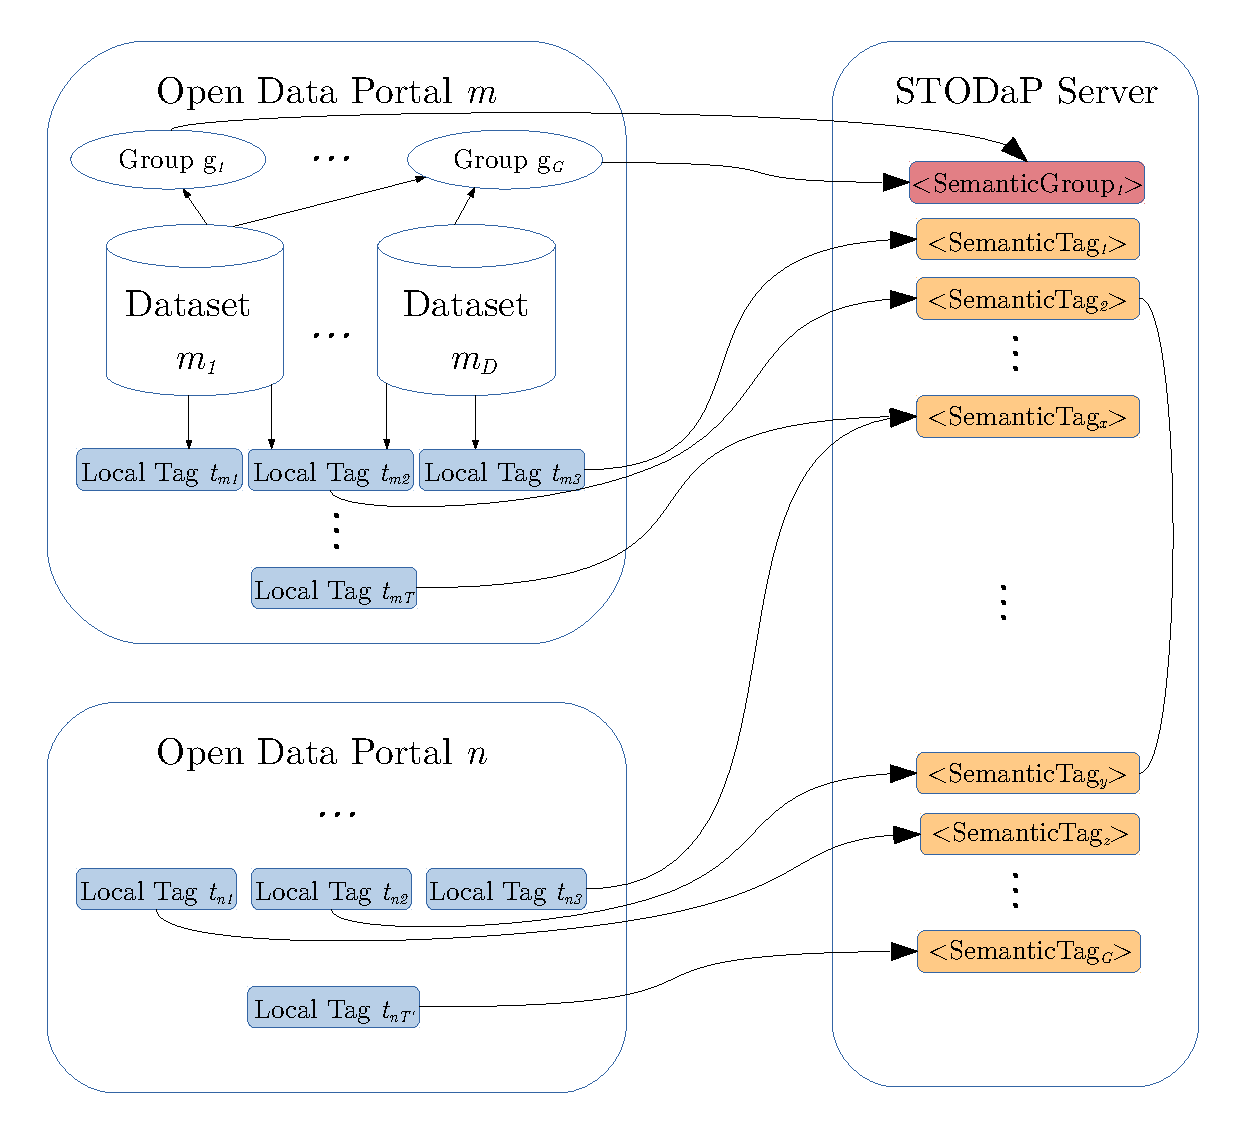
\includegraphics[scale=0.6]{images/odp_definition.pdf}
\caption{Relevant elements of the Semantic Tags for Open Data Portals system.}
\label{fig:definition}
\end{center}
\end{figure}


%#########################################################################################
\section{Overview of the STODaP Approach}
\label{sec:stodap_overview}
%#########################################################################################

In this section, we give an overview on the tag reconciliation approach for cleaning up and connecting ODPs, supported by software tools both at the local and global contexts.
The objective of the approach is to tackle the main problems identified by the metrics described in the previous section, and thus to facilitate data organization and linking through metadata descriptions of ODPs.

Figure \ref{fig:overview}\footnote{Icons by \href{http://www.flaticon.com/authors/simpleicon}{SimpleIcon} from \href{http://www.flaticon.com}{www.flaticon.com} are licensed under \href{http://creativecommons.org/licenses/by/3.0/}{CC BY 3.0}.} shows an overview of the proposed approach.
Data publishers in charge of ODPs are offered tools for local tag curation.
These tags are then connected to global tags hosted in a central Tag Server, which can be collaboratively edited both by data consumers and publishers. 
They can add new semantic descriptions to the global tags, establish relations between them, and also create new links between global and local tags.
Data consumers have the option to retrieve data directly from ODPs, or through references gathered from the central server.
%The description of these actions is shown in the sequel.

\begin{figure*}[tb]
\begin{center}
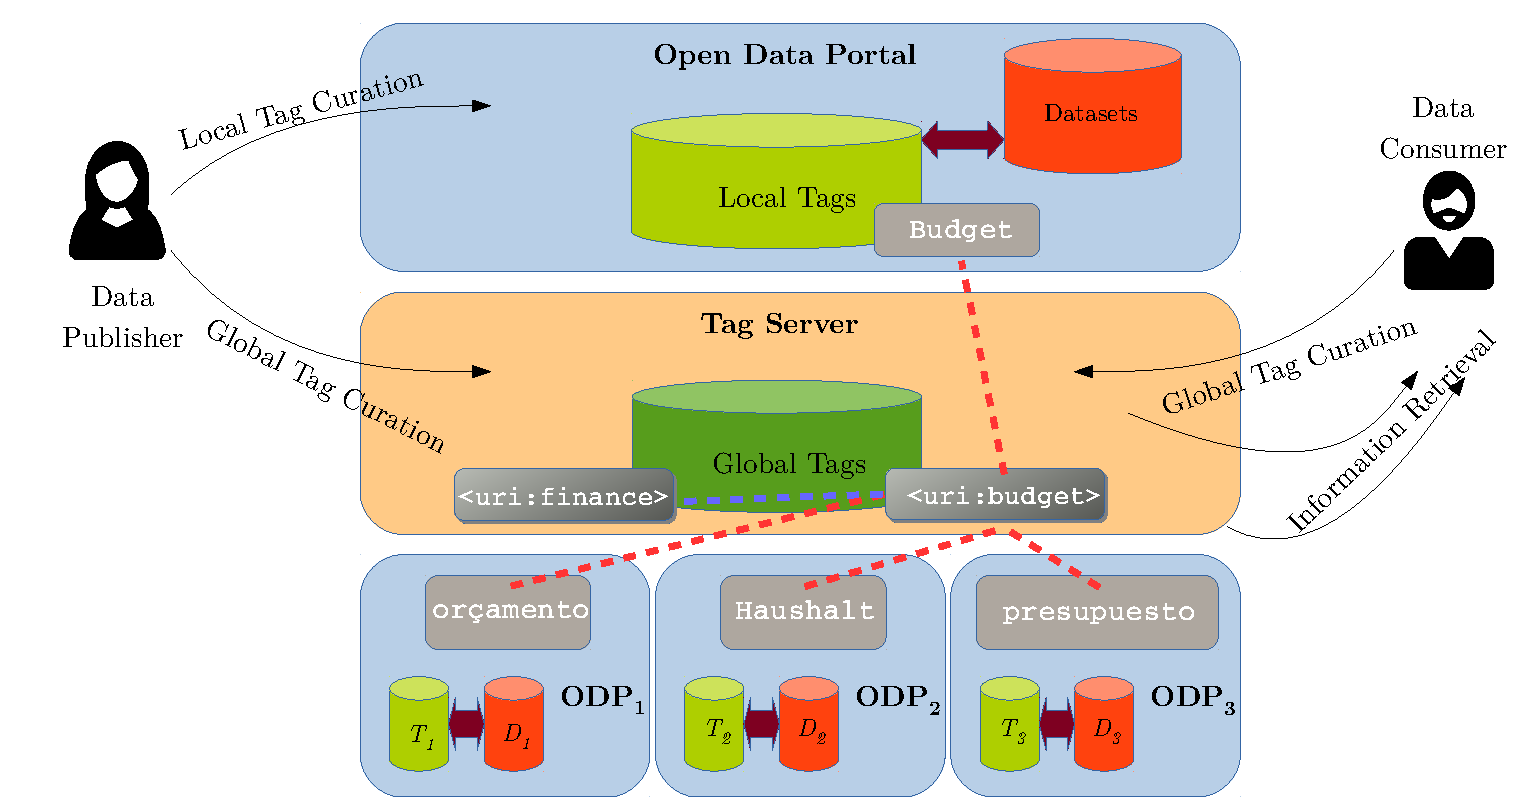
\includegraphics[scale=0.65]{images/overview.pdf}
\caption[Overview of the StodAp approach.]{Overview of the StodAp approach. Local tags are connected to a corresponding global tag within a central tag server. 
Data managers responsible for ODPs may use tools for local tag curation, as well for maintaining the tag server. 
This task is also expected to be performed by data consumers.}
\label{fig:overview}
\end{center}
\end{figure*}

The following three sections are dedicated to further detail the approach.
Section \ref{sec:stodap_building} explains the procedure used to build the first version of the semantic tag server.
In the following, Section \ref{sec:use_and_maintenance} describes the STODaP tools and methodologies for open data managers and users in order to maintain the tag server.
Finally, \autoref{sec:implementation} describes the implementation of the tools.

%#########################################################################################
\section{Building the STODaP server}
\label{sec:stodap_building}
%#########################################################################################

In order to build the first version of the STODaP server, a tag harvesting was done through 87 ODPs.
Almost 300.000 tags were processed, using their names and informations as language and groups that the tagged datasets belong to.
In the following, we describe first the procedures for the individual portals, and then the procedures for whole tag set until we come to the structured Global Tag Set.

\subsection{Local Processing - Clean Up and Reconcile}
\label{sec:local_building}

An overview of the procedure applied locally, i.e., for each ODP, is shown in \autoref{fig:local_processing}.
In the figure, each green block represents a processing phase, which is materialised in a set of tag representations. 
The grey blocks describe the transformations suffered by the tag sets from one phase to another.
The aim of the local processing steps is to transform freely written tags into semantic resources that are candidates for representing the datasets they are associated.
Each transformation applied to the tags on the local processing is detailed bellow:

\begin{figure*}[tb]
\begin{center}
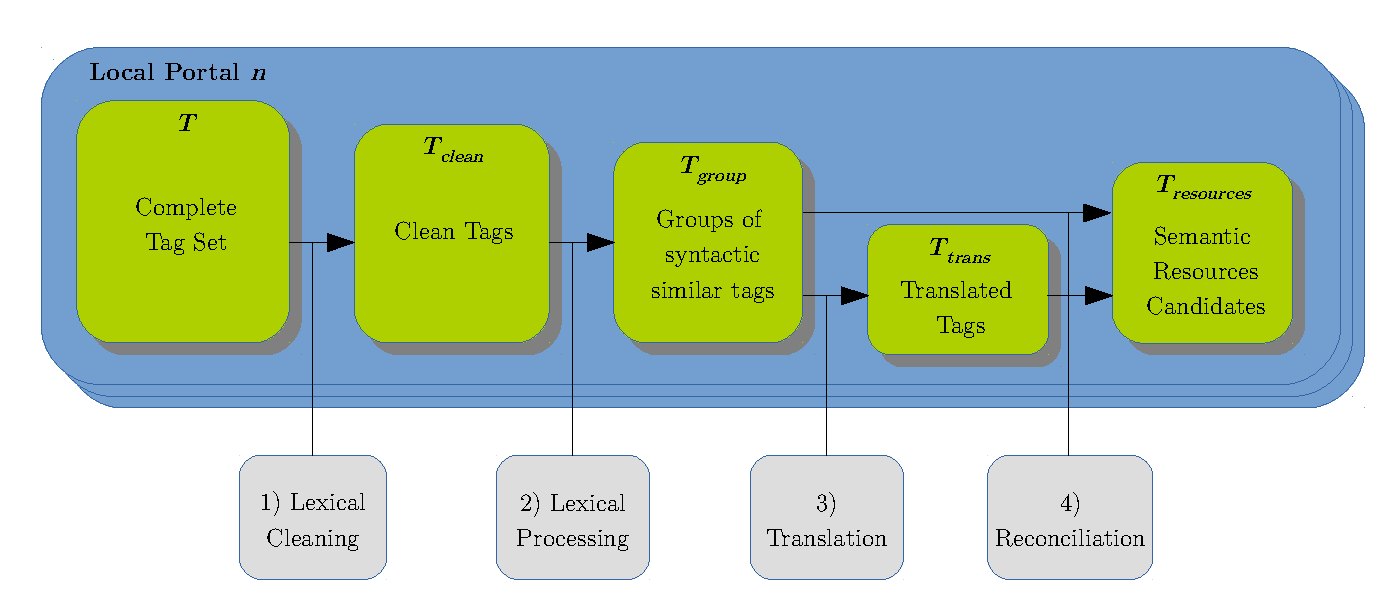
\includegraphics[scale=0.7]{images/local_processing.pdf}
\caption[Overview of the local tag processing.]{Overview of the local tag processing.}
\label{fig:local_processing}
\end{center}
\end{figure*}

\noindent \textbf{Lexical Cleaning: }The complete tag set $T$ is the set containing all original tags found in one portal.
Firstly, the \emph{Lexical Cleaning} is applied in order to discard tags with low probability of getting a semantic meaning.
At this point, some heuristics are applied, and a tag is discarded if it is: 
\begin{itemize}
	\item smaller than 4 characters; 
	\item composed of numbers and alphabetic characters;
	\item exclusively composed by uppercase characters;
	\item not started by a alphanumerical character;
	\item larger than 5 words; or
	\item not applied to any dataset.
\end{itemize}

\noindent \textbf{Lexical Processing:} After the Lexical Cleaning, we have the resulting set $T_{clean}$ of clean tags, with a higher probability of being reconciled with semantic concepts in ontologies.
The following procedure is the \emph{Lexical Processing}, which aims to group tags that have a lexical similarity.
These similar tags have a high probability of representing the same meaning, with small lexical variations.
In order to determine this similarity, we apply the Levenshtein edit-distance to the lowercased and unaccented tags (which means that \texttt{Açaí} will be transformed into \texttt{acai} before measuring the distance).
Based on manual experimentation, we consider that tags with an edit-distance of 0 or 1 are similar.
This distance captures plural, gender and temporal variations in most of the languages present in our sample.
The proceeding results in the set $T_{group}$ of syntactically similar tags.

\noindent \textbf{Translation:} The sample used to build this tag server contains portals in 22 different languages.
Thus, it is necessary to use translation services on the Web to transform words from their original language to the English language.
English language was chosen because of the higher availability of translation services, and also because the main ontologies have their terms described necessarily in English, and possibly also in other languages.
It also significant that 43\% of the portals are in English (according to the provided metadata), and their tags represent 83\% of all tags.
Each group of similar tags from $T_{group}$ was translated, resulting possibly in a set of translations for each group.
The new set achieved in this processing is $T_{trans}$.

\noindent \textbf{Reconciliation:} The previous proceeding results in a set $T_{trans}$ of groups formed by all the related translations.
Until this moment, we were dealing with string of characters.
In this stage, these names will be the input for searching semantic representations for the tags.
In order to get the widest spectrum of possibilities, the search for semantic resources is done for all lexical representations of the tag, stored in $T_{group}$, and also all possible translations of it in $T_{trans}$.
The resulting set will be denominated $T_{resources}$.

%The product of this step are synonym rings, or synsets, where the groups of words have are semantically equivalent for the purpose of retrieving information.
%The proceeding results in the set $T_{synt\_sem}$ of semantically similar tags.

%Finally, in order to prepare the tags for linking with other portals, we come to the \emph{Translation} step.
%Each tag is translated to the English language, forming the set $T_{english}$ of translated tags.
%->> tentar todas as opções de tradução
In order to illustrate the procedure, \autoref{tab:local_example} shows an example using real tags from the Brazilian Data.gov.br.
From $T$ to $T_{clean}$, tags containing numbers, too small or representing abbreviations were removed.
Then, similar tags were grouped to form $T_{group}$.
The translation process could not find an equivalent for the first group.
Even so, the semantic search-engine was able to find a matching resource for \texttt{Acidente de trabalho} (accident at work), as well as for the other two.

\begin{table}[]
\centering
\ABNTEXfontereduzida
\caption{Examples of tags in each step of the procedure.}
\label{tab:local_example}
\begin{tabular}{|p{2cm}|p{2cm}|p{2cm}|p{2cm}|p{2cm}|p{2cm}|}
\hline
$T$ & $T_{clean}$ & $T_{group}$ & $T_{trans}$ & $T_{resources}$ \\ \hline
Acidente de trabalho,
Acidentes de trabalho,
CNAE,
finanças,
Folha SA.23,
Folha SB.23 
município,
orçamento,
UF
&
Acidente de trabalho,
Acidentes de trabalho,
finanças,
orçamento
&
\{Acidente de trabalho, Acidentes de trabalho\}
finanças,
orçamento
&
--
finances,
budget
&
\{gemet:9366, eurovoc:825\},
eionet:3194
eionet:1025 \\ \hline
\end{tabular}
\end{table}

It is important to notice that the process described above is subject to several failures.
On the Lexical Cleaning step, meaningful tags with less than 4 characters may be discarded, as well as unintentionally uppercased words.
On the Lexical Processing stage, it is possible that in some languages the same word starting with capital and non-capital letters have different meanings.
With a higher probability, words differing from edit-distance of 2 may also have different (or even opposed) meanings, such as \texttt{child-death} and \texttt{child-health}, found on data.gov.uk.
On the Translation phase, the main problem lies on polysemy, where the same word has several meanings.
While also heavily dependent on the translation tools, providing side tags or other metadata can help the algorithm finding the right translation.
Finally, when searching for the meanings, there is a great dependency on the tool used and the available knowledge bases.

\subsection{Global Processing - Interlinking Portals}
\label{sec:global_building}

After reaching the last stage of the local processing stage for each one of the 87 portals, a joint process starts over $T_{resources}$ in order to build the Semantic Tag Server.
At the global processing stage, there are three main steps:

\begin{enumerate}
	\item Select meaningful tags;
	\item Create global tags and connect local tags to them; and
	\item Discover and qualify relations between tags.
\end{enumerate}

In order to accomplish this objective, we propose the global procedure shown in Figure~\ref{fig:global_processing}.

\noindent \textbf{Significance Selection: } We start the global processing with a joint set $\mathcal{T}_{resources}$, which contains $T_{resources}$ from all portals. 
In this set, a \emph{Significance Selection} process is driven, in order to determine tags that will be useful on the information retrieval process.
This is an heuristics based process, which considers: (i) Success on finding semantic candidates for the tag; (ii) the number of datasets pointed by this tags; (iii) the quality of the semantic resources candidates.

\noindent \textbf{Semantic Processing:} After this step, the Global Tags will be derived.
Global Tags are semantics entities, who have a main name in English, several translations, and point to local tags, which in turn connect to datasets located into Open Data Portals.

\noindent \textbf{Structure Emergence:} Finally, relations between Global Tags in set $G$ will be searched on the ontologies they appear in order give a structure to the Global Tag set $G_{struct}$.
The first strategy is to search for relations on the reconciled ontologies, and set this relation between the global tags.
Thus, relations as \texttt{skos:related}, \texttt{skos:narrower} and \texttt{skos:broader} can be set.
However, at this point we notice need of an upper classification scheme.

The ODP model, as shown in \autoref{fig:definition}, includes a Group element, to which one or more datasets can be associated.
Thus, it is possible to consider that a tag associated to a dataset which is in a group is also related to this group.
However, only 11\% of all datasets in our sample are associated to groups, and only 13\% of the tags are associated to datasets in groups.

If we look to some ODPs which are organized in groups, it is possible to see a similar organization.
In \autoref{tab:groups}, we list the groups of 4 ODPs. 
If we look at the table, it is clear that in the context of open government data portals, there are some specific categories, but the portals also share common subjects, such as Health, Education or Culture.

\begin{table}[]
\centering
\ABNTEXfontereduzida
\caption{Examples of groups in some ODPs}
\label{tab:groups}
\begin{tabular}{|p{3.2cm}|p{3.2cm}|p{3.2cm}|p{3.4cm}|}
\hline
Data.gov & Data.gov.de & Dados.gov.br & Data.buenosaires.gob.ar \\ \hline
Aging / Agriculture / Business / Climate / Consumer / Disasters / Ecosystems / Education / Energy / Finance / Health / Law / Local Government / Manufacturing / Ocean / Public Safety / Science \& Research &
Population / Education and science / Geography, Geology and the GEODATA / Laws and justice / Health / Infrastructure, building and housing / Culture, leisure, sport, tourism / Not yet categorized / Public administration, budget and taxes / Politics and elections / Social / Transport and traffic / Environment and the climate / Consumer protection / Economy and work &
Municipal Chamber
/ trade, services and tourism
/ culture, leisure and sport
/ data sets in the spotlight
/ defence and security
/ economy and finance
/ education
/ public facilities
/ geography
/ government and politics
/ housing, sanitation and urbanism
/ health information
/ industry
/ justice and law
/ environment
/ person, family and society
/ management platform indicators
/ multi-year plan
/ international relations
/ health
/ work
/ transportation and transit &
economic activity /
public administration and policy /
culture and recreation /
education /
infrastructure and public works /
environment /
mobility and transport /
health and social services /
security /
urbanism and territory \\\hline
\end{tabular}
\end{table}

Thus, after translating all the group names, we verified that 62 group names occurred in three or more portals.
These were chosen as the first Global Groups.
The second step consisted in verifying the lexical similarity between all groups and the Global Groups in order to associate groups with Global Groups.
Some distortions were observed, such as \texttt{sport} being associated with \texttt{transport}, or \texttt{culture} with \texttt{agriculture}.
These errors were manually corrected.

Finally, groups were reconciled with general-purpose ontologies.
Particularly, the Gemet Thesaurus\footnote{Available at \url{http://www.eionet.europa.eu/gemet/}} fits well for this purpose.

%All Datasets: 470551
%Datasets in Groups: 53158
%Tags in Groups: 37743

\begin{figure*}[tb]
\begin{center}
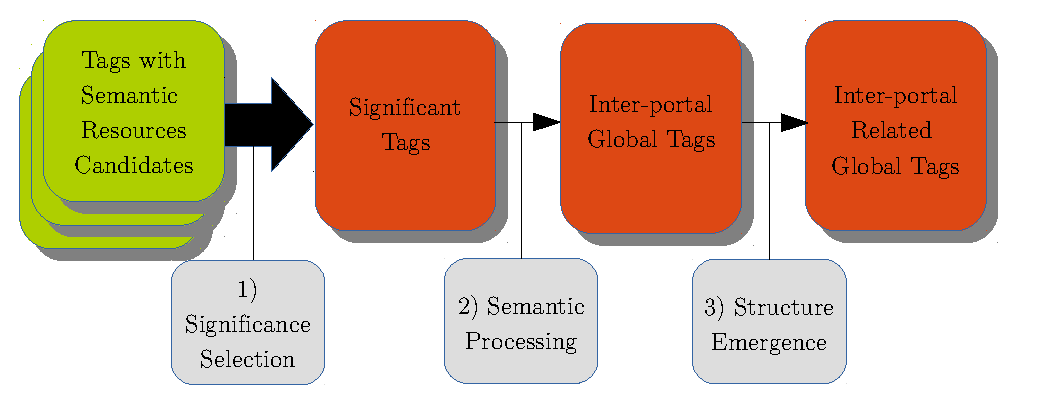
\includegraphics[scale=0.8]{images/global_processing.pdf}
\caption[Overview of the local tag processing.]{Overview of the global tag processing.}
\label{fig:global_processing}
\end{center}
\end{figure*}

%#########################################################################################
\section{Use and Maintenance of the STODaP server}
\label{sec:use_and_maintenance}
%#########################################################################################



After building the Semantic Tag Server (STODaP), it is necessary to maintain and enhance the tag corpus alongside the evolution of ODPs, as well as to maintain the server updated.
In this subsection, the strategy for it will be presented, locally and globally at the individual portal level, and at the server level.


\subsection{Local Part - Cleaning up tags}
\label{sec:local}

Section \ref{sec:local_metrics} showed that ODPs suffer from low reuse of tags, and that there is a significant tags duplication due to slight spelling differences. 
In fact, both problems -- low reuse and duplication -- are connected, since merging similar tags improves tag reuse.
However, low tag reuse can be also attributed to the lack absence of a standard tagging procedure, which would guide users in this task.

To address this problem locally at a particular ODP, we propose an approach for reconciliation of tags. %, and for enhancing the quality of the new ones.

First, we offer three levels of semi-automatic tag merging strategies:

% spell 
% check for sem similatyy libs in phyton

\begin{enumerate}
	\item With high confidence, we suggest merging tags that differ only by capital letters or special characters. 
In many ODPs, this strategy will already achieve significant results, as shown in Figure~\ref{fig:similarity}.
	\item After running the first strategy, the Levenshtein distance is computed for all remaining pairs of tags.
Tags with distance one or two are suggested for merging, in order to catch plural/gender variations, such as \texttt{worker} and \texttt{workers}. 
However, false-positives like \texttt{widow} and \texttt{window} may appear.
Tags composed only by numbers (to avoid merging tags representing years) or less than 4 characters are not included.
	\item Finally, we use semantic measures~\cite{Harispe01032014} to determine the semantic similarity between two tags. 
In this case, the tags \texttt{autumn} and \texttt{fall} have a high similarity, and thus will be suggested for merging.
\end{enumerate}

%For the new tags, besides suggesting tags that were already used in the portal, we also suggest tags based on the previous tags (and on the context???). 
It must be noted that all these approaches have originally quadratic time complexity, because every pair of tags has to be computed. However, sorting tags alphabetically turns the problem into linear in strategies 1 and 2 (however, with possible losses in 2), and ignoring tags without correspondence in dictionary reduces the dimension in strategy 3.

After this cleaning procedure, we offer users the opportunity to link each local tag to a global correspondent at the tag server, described in the sequel.
%TODO improve here

\subsection{Global Part - Semantifying Tags}
\label{sec:global}

% add new portal
% renew portal

With the aim of building a common and collaborative basis for interlinking ODPs, we developed a Global Tag Server.
The conceptual rationale is:
\begin{enumerate}
	\item To assist individual ODPs enhancing the quality of their tags, by assigning a common agreed meaning to them;
	\item To create a collaborative platform for meaningfully linking ODPs.
\end{enumerate}

The Global Tag Server hosts the description of global tags.
Each global tag may be associated to one or more Linked Open Data resources, representing their semantic meanings.
Linking to the local tags is accomplished via the URIs which represent a local tag in its context.
The global tags can also have several types of relations between each other, such as \texttt{skos:broader}, \texttt{skos:narrower} or \texttt{owl:sameAs}.
Figure \ref{fig:example} illustrates the concept with an example.

\begin{figure}[tb]
\begin{center}
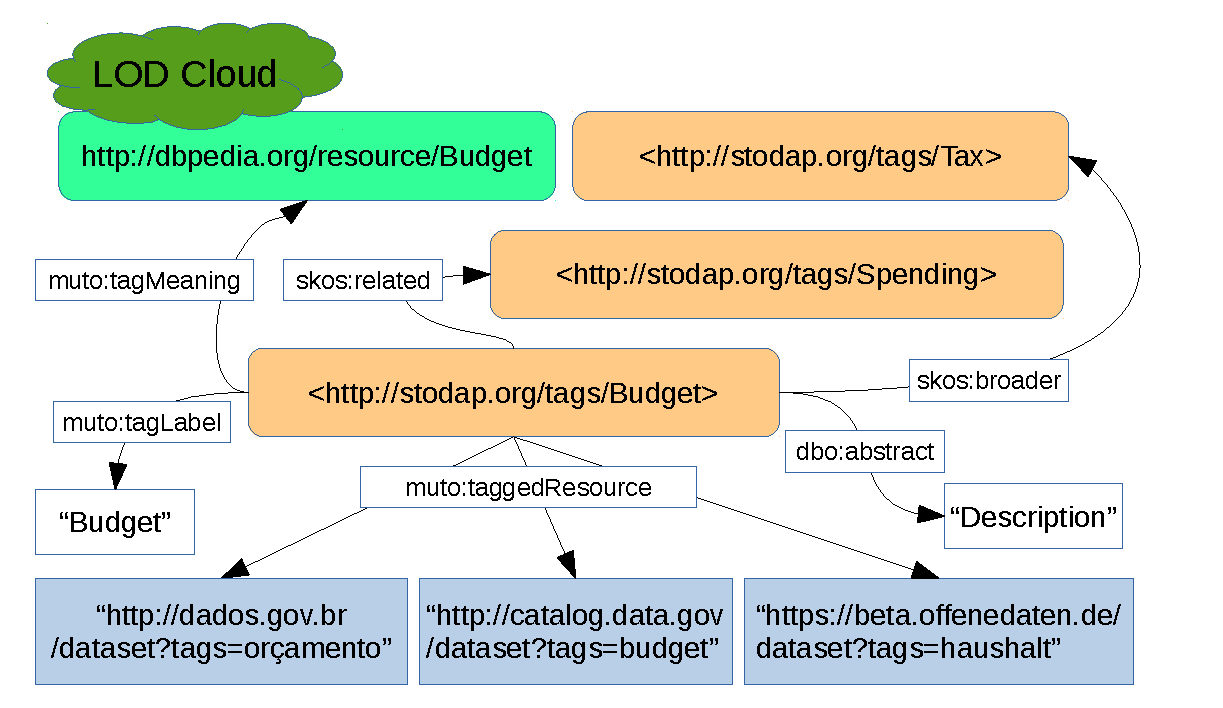
\includegraphics[scale=.7]{images/example.pdf}
\caption{Example of the STODaP model showing relationships of the global tag \url{http://stodap.org/tags/Budget}.}
\label{fig:example}
\end{center}
\end{figure}

The example shows the global tag identified by the URI \texttt{<http://stodap.org/tags/Budget>}. 
With this global tag, a meaning and some URIs of local tags are associated.
The global tag is also semantically related to other global tags, using the SKOS vocabulary.
The MUTO ontology\footnote{\url{http://muto.socialtagging.org/core/v1.html}} is used to define some concepts and relations between the tags, like \texttt{muto:Tag}, \texttt{muto:taggedResource}, \texttt{muto:hasTag} and \texttt{muto:hasMeaning}.

\subsection{STODaP Server - Interlinking Portals}

The first step for building the semantic tag server is to harvest metadata from open data portals.
After the initial setup, a strategy for maintaining the portal up-to-date is needed.

\textbf{Adding a new portal}

When a new ODP is added to the system, a setup procedure is followed:
\begin{itemize}
	\item Harvest tags, datasets and groups metadata;
	\item Clean and group similar tag;
	\item Translate tags, in case of non-English portal;
	\item Reconcile tags with existing Global Tags;
	\item If reconciliation is not successful, search lexvo.org and try to create a new global tag;
	\item Groups: reconcile with existing global groups or create new ones.
\end{itemize}

\textbf{Updating a portal}

When an ODP is updated, the procedure followed is:
\begin{itemize}
	\item Harvest tags, datasets and groups metadata;
	\item Verify which datasets were inserted or modified
\end{itemize}

%#########################################################################################
\section{Implementation}
\label{sec:implementation}
%#########################################################################################

In this section, we detail the technical procedures related to the previous sections.
We first describe the implementation of the procedure for discovering the Global Tags, discussed in \autoref{sec:stodap_building}.
Then, we describe the implementation of two CKAN plugins:
(i) \emph{CKAN Tag Manager}\footnote{\url{https://github.com/alantygel/ckanext-tagmanager}} and 
(ii) \emph{CKAN Semantic Tags}\footnote{\url{https://github.com/alantygel/ckanext-semantictags}}, which materialize the ideas reported in \autoref{sec:use_and_maintenance}.
Finally, we describe the implementation of the Semantic Tag Server for Open Data Portals.

\subsection{Building Global Tags}

\begin{itemize}
	\item Harvest all tags from portals
	\item Filter significant tags
	\item Group syntactically similar
	\item Translate - lexvo + yandex
	\item Reconcile - lexvo - several ontologies
	\item Choose gemet tags and create global tags and links
	\item Create global groups, and reconcile
	\item Associate global tags to global groups

	
\end{itemize}

\subsection{CKAN Tag Manager Plugin}

The CKAN Tag Manager one offers an environment for tag curation directly inside the CKAN platform. 
It comprises basic functions such as deletion and editing of tags, and advanced function aimed to enhance the quality of tags.
In this sense, the plugin checks:
\begin{itemize}
	\item Very similar tags, differing by capitals or special characters;
	\item Similar tags, with a Levenshtein distance $\le 2$ (after lowercasing and unaccenting)
	\item Possible synonyms, using Natural Language Toolkit~\cite{Bird2009}.
\end{itemize}
In all those cases, the user is offered the option of merging the respective pair of tags. 
\autoref{fig:local_curation} shows a screenshot of the CKAN Tag Manager.

\begin{figure}[tb]
\begin{center}
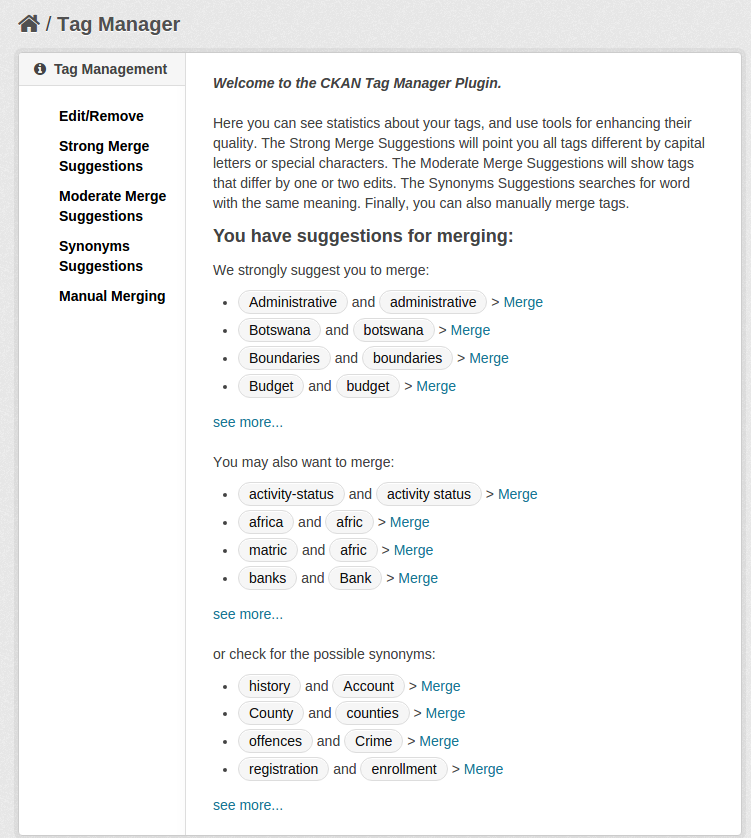
\includegraphics[width=\columnwidth]{images/local_curation.png}
\caption[Local tag curation in a CKAN instance.]{Local tag curation in a CKAN instance. The plugin offers possibilities of manual and semi-automatic tag merging. The first block contains only valid suggestions, while the second block shows 2 false-positives. The synonym module also detected plurals. Tags in this example were extracted from the africaopendata.org portal.}
\label{fig:local_curation}
\end{center}
\end{figure}

\subsection{CKAN Semantic Tags Plugin}

The CKAN Semantic Tags plugin implements the connection between a CKAN instance and the Global Tag Server.
Each local tag can be associated to a global tag from the server.
After the association, datasets linked with a local tag also point to the global server, as shown in \autoref{fig:local_link}.

\begin{figure}[ht]
\begin{center}
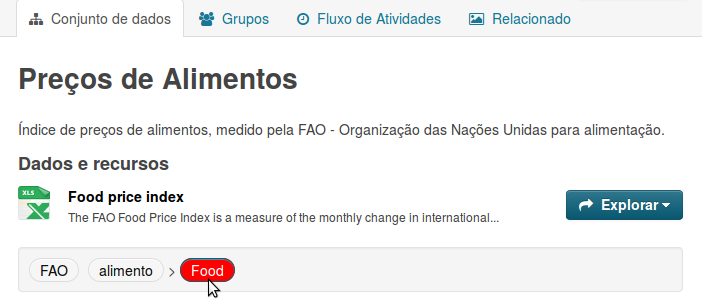
\includegraphics[scale=.5]{images/local_link.png}
\caption[Detail of dataset in an ODP.]{Detail of dataset in an ODP. The dataset is tagged with two tags, and one of them (\texttt{alimentos}) is connected to the global tag \texttt{http://stodap.org/tags/Food} through the \texttt{muto:hasTag} property.}
\label{fig:local_link}
\end{center}
\end{figure}

\subsection{Semantic Tag Server}

The tag server is implemented using the collaborative \emph{MediaWiki}. 
Specially, the \emph{Semantic MediaWiki} extension~\cite{Kroetzsch2007} is used in order to include properties and integrate the global tags in the LOD Cloud, through the export of RDF files.
The page of a global tag is shown in \autoref{fig:tag_server}.
Each global tag page is build using \href{https://www.mediawiki.org/wiki/Extension:Semantic_Forms}{semantic templates and forms}, in order to facilitate consistency and coherency and to be more user-friendly.

\begin{figure}[ht]
\begin{center}
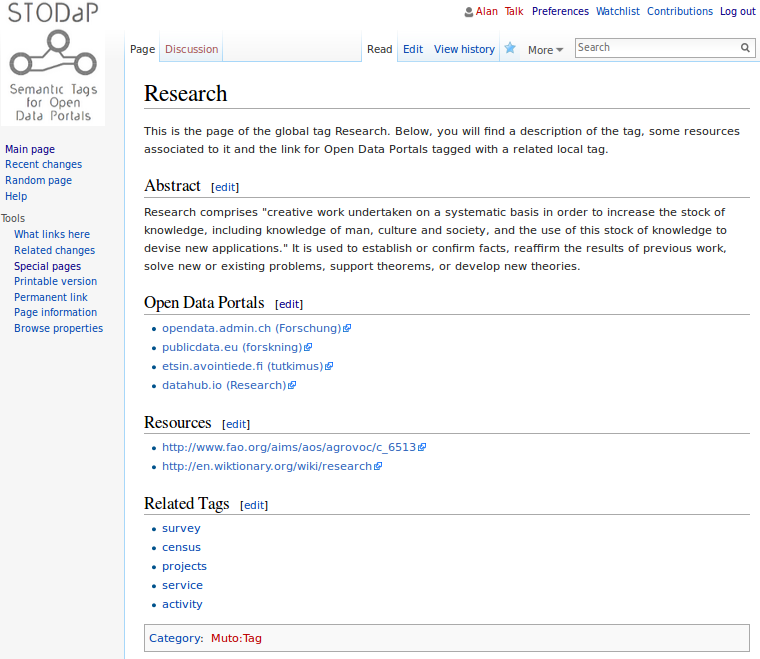
\includegraphics[width=\columnwidth]{images/tag_server.png}
\caption[Semantic Tag Server for Open Data Portals.]{Semantic Tag Server for Open Data Portals. Simplified example of the global tag \texttt{Research}, which is linked to 48 Open Data Portals and 16 semantic resources. In the screenshot, we illustrate a few of them.}
\label{fig:tag_server}
\end{center}
\end{figure}

%#########################################################################################
\section{Results}
\label{sec:results}
%#########################################################################################

We describe in this section some results achieved with the STODaP approach.
At the global level, it was possible to implement the global tags server and to test the performance.
%At the local level it is only possible to claim potential results, as we do not have access to the single ODPs.

\subsection{STODaP Server}

In order to test the system, an open-source implementation of STODaP was created and deployed at \url{http://stodap.org}.
The following approach was used create 663 global tags at the server:
\begin{itemize}
	\item From the 220,567 tags harvested, we selected the 663 that were used in more portals, representing all tags used in 10 or more portals; 
	\item Using the Lexvo.org service, we found URI candidates to represent the tag meaning via the \texttt{lexvo:means} property;
	\item Using the Lexvo.org service, we found translations and synonyms for the tags via the \texttt{rdf:seeAlso} and \texttt{lexvo:translate} properties;
	\item We searched for the translations and synonyms in the harvested tags and included the results as \texttt{muto:taggedResources}, together with the portals tagged with the original term;
	\item Using the \href{http://www.nltk.org/}{Natural Language Toolkit  Library}, we searched for semantic similar global tags, which were added as \texttt{skos:related}.
\end{itemize}

The occurrence of the original tags among the portals, and the results after including the translations and synonyms can be seen in \autoref{fig:results_tagged_resources}. 
The graphic shows the 30 most used tags, and the achieved increment in the number of relations. 
The occurrence of tags denoting years can also be noticed.
Obviously these tags have no synonyms nor translations, and thus no increment is shown. 
It is also worth mentioning that the tag \texttt{{test}} is the fourth most used one.
This fact is probably related to the early stage of development of some portals. 

\begin{figure}[tb]
\begin{center}
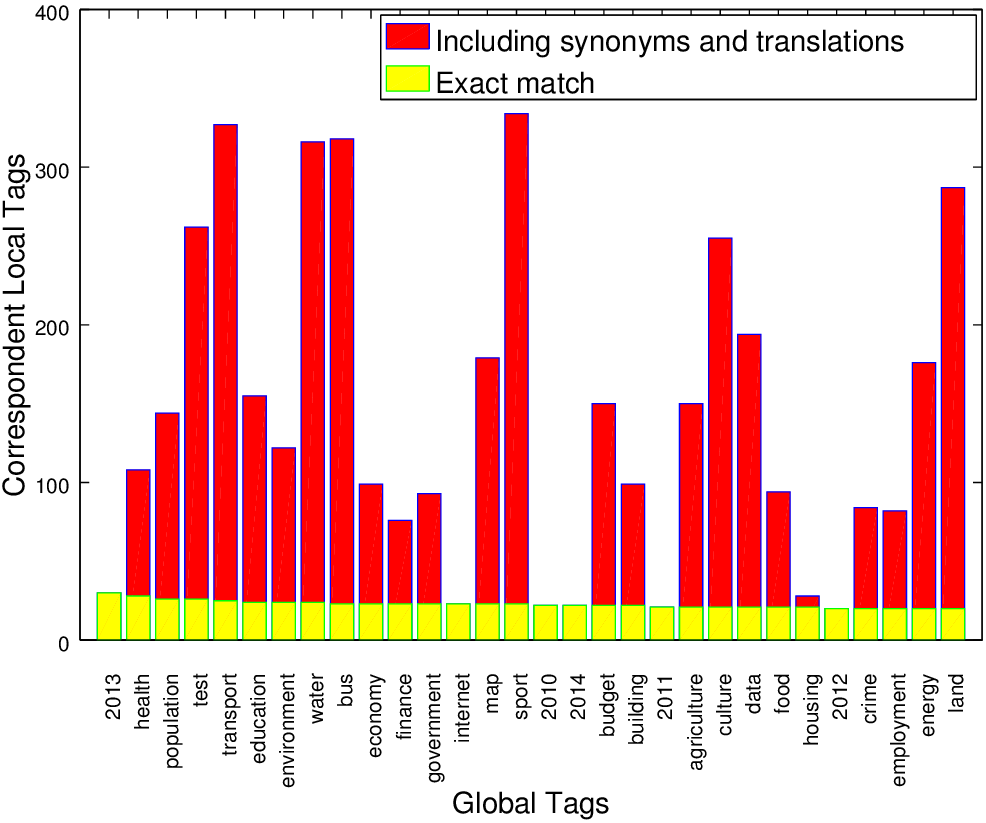
\includegraphics[scale=.8]{images/results_tagged_resources.png}
\caption{Correspondence between local and global tags. The yellow bar shows the number of exact occurrences of the tag in ODPs. The red bar shows the improvement when considered translations and synonyms, which can also occur in a same portal. This explains the numbers over 90. }
\label{fig:results_tagged_resources}
\end{center}
\end{figure}

\subsection{Local Level}

At the local level, the main potential achievements are at the tag curation process.
As shown in \autoref{fig:similarity}, a considerable number of pairs of tags differ only by capital or accented characters.
Using the naive approach to merge similar tags in every portal would result in reducing the number of 14,168 local tags, which represents 6.4\% of the total number of tags.
Lowercase and unaccented tags differing by a Levenshtein-distance from 0 to 2 represent a total of 35,066 pairs, or 15,8\% from the whole tag universe.
However, as discussed above, this approach can lead to false-positives and thus requires manual checking.


%#########################################################################################
\section{Conclusions}
\label{sec:stodap_conclusions}
%#########################################################################################

In this chapter, we presented an approach for metadata reconciliation within and among Open Data Portals.
The use of tags was analysed, and several problems were found, such as a low tag reuse rate and the overall existence of different tags for the same meaning.
On the analysis we also found that several portals share the same tags, showing that tags have a good potential to be linking elements among datasets.
Converting tags into semantic identifiers was also shown as a viable option, even though more sophisticated methods have to be investigated. 
Based on these findings, we derived the STODaP approach, which comprises two parts: 
a local one, aimed at cleaning up and enhancing the quality of ODPs tags, and 
a global one, for connecting ODPs through semantic tags.
The implementation of both shows that significant enhancements can be achieved both at the individual ODPs and the global levels.

Future research and development includes a tag suggestion approach for ODPs which takes into account the related tags at the tag server, using collective knowledge as in~\citeonline{Sigurbjornsson2008}.
Using the possibly structured data of the ODPs in order to improve tagging suggestions is also a research direction that should be followed.
At the global level, an interesting approach is to detect the emergence of schemas from the tags, as described in~\citeonline{Robu2009}.
We will also call for the attention of the open data community in order further to advance collaborative strategies for enriching the tag server.
For STODaP to realize its full potential, ODP administrators and users should be involved and (meta)data literacy needs to be improved.

The ``openness'' of open data is still limited by many factors, including politics, data literacy and technology ones.
With this work, we contributed to the organization and interconnection of ODPs, and thus, given a step further on the enhancement of the open data field.


%1) juntar grupos 
%2) ver quantas tags e datasets estão la dentro
%3) dentro de cada grupo organizar melhor

%Categorization: http://eurovoc.europa.eu/drupal/?q=navigation&cl=en
%Categorization: http://www.eionet.europa.eu/gemet/

